\documentclass[a4paper, 12pt]{article}
\usepackage{a4wide}
\usepackage {amsmath}
\usepackage {graphicx}
\usepackage[utf8]{inputenc} 
\usepackage[francais]{babel}
\usepackage{fancyhdr}
\usepackage{setspace}
\usepackage{fancyhdr}
\usepackage{lastpage}
\usepackage{extramarks}
\usepackage{chngpage}
\usepackage{soul}
\usepackage[usenames,dvipsnames]{color}
\usepackage{graphicx,float,wrapfig}
\usepackage{ifthen}
\usepackage{listings}
\usepackage{courier}
\usepackage{esint}
\usepackage{bbm}
\usepackage{graphics}
\usepackage{graphicx}
\usepackage{subfig}
\usepackage{epsfig}
\usepackage{pgf,tikz}
\usetikzlibrary{arrows}
\usepackage{braket}
\usepackage{MnSymbol,wasysym}
\usepackage{marvosym}
\usepackage{dsfont}
\usepackage{esdiff}
\usepackage{cancel}
\usepackage{wrapfig}
\usepackage{color}
\usepackage{etoolbox}

\usetikzlibrary{decorations.pathmorphing,patterns}

\newtoggle{CORR}
\toggletrue{CORR}   
% \togglefalse{CORR}

\lhead{} 
\chead{} 
\rhead{\bfseries $\theta$-schéma} 
\lfoot{JC Toussaint}
%\cfoot{} 
%\rfoot{\thepage}

% This is the color used for MATLAB comments below
\definecolor{MyDarkGreen}{rgb}{0.0,0.4,0.0}

% For faster processing, load Matlab syntax for listings
\lstloadlanguages{Matlab}%
\lstset{language=Matlab,                        % Use MATLAB
        frame=single,                           % Single frame around code
        basicstyle=\small\ttfamily,             % Use small true type font
        keywordstyle=[1]\color{Blue}\bf,        % MATLAB functions bold and blue
        keywordstyle=[2]\color{Purple},         % MATLAB function arguments purple
        keywordstyle=[3]\color{Blue}\underbar,  % User functions underlined and blue
        identifierstyle=,                       % Nothing special about identifiers
                                                % Comments small dark green courier
        commentstyle=\usefont{T1}{pcr}{m}{sl}\color{MyDarkGreen}\small,
        stringstyle=\color{Purple},             % Strings are purple
        showstringspaces=false,                 % Don't put marks in string spaces
        tabsize=5,                              % 5 spaces per tab
        %
        %%% Put standard MATLAB functions not included in the default
        %%% language here
        morekeywords={xlim,ylim,var,alpha,factorial,poissrnd,normpdf,normcdf},
        %
        %%% Put MATLAB function parameters here
        morekeywords=[2]{on, off, interp},
        %
        %%% Put user defined functions here
        morekeywords=[3]{FindESS, homework_example},
        %
        morecomment=[l][\color{Blue}]{...},     % Line continuation (...) like blue comment
        numbers=left,                           % Line numbers on left
        firstnumber=1,                          % Line numbers start with line 1
        numberstyle=\tiny\color{Blue},          % Line numbers are blue
        stepnumber=5                            % Line numbers go in steps of 5
        }

% Includes a MATLAB script.
% The first parameter is the label, which also is the name of the script
%   without the .m.
% The second parameter is the optional caption.
\newcommand{\matlabscript}[2]
  {\begin{itemize}\item[]\lstinputlisting[caption=#2,label=#1]{#1.m}\end{itemize}}

\pagestyle{fancy}

\begin{document}

\bibliographystyle{alpha}

\title{Intégration numérique d'une équation différentielle}

%\author{Jean-Christophe Toussaint\\
%  Phelma\\
%\texttt{jean-christophe.toussaint@phelma.grenoble-inp.fr}
%}
\date{\today}
 
\maketitle

\section{Intégrateurs à pas adaptatif}

On présente ici une famille de méthodes d'intégration des équations différentielles plus  versatile gérant elle-même le choix
du pas de temps d’intégration $h$. 

L'utilisateur doit d'abord bien connaître la physique du problème qu'il traite car 
il doit définir une valeur acceptable $\epsilon_m$ de l'erreur d'intégration
à chaque pas. 

A chaque itération, l'idée principale est d’ajuster le pas d’intégration de manière 
à ce que l’erreur $\epsilon$ ne dépasse pas la valeur de l’erreur acceptable $\epsilon_m$.
L'algorithme consiste à d’effectuer l’intégration du système d’équations différentielles de l’instant $t_n$ à l’instant $t_n+h$, deux fois avec 
 deux méthodes différentes, la seconde étant d'un ordre de précision supérieur à la première.

Chacune donne une estimation de $Y(t_n+h)$ que l’on note $A_1$ et $A_2$ qui nous servirons à
calculer une estimation de l’erreur commise lors de l’intégration.

\subsection{Méthode d'Euler à 2 pas}

Pour notre démonstration, on suppose connaître la fonction $\Phi(t)$, solution analytique de notre système d'équations
 différentielles $\frac{dY}{dt} = f(t, Y)$.

Sans perdre en généralité, on suppose qu'à l'instant $n$, les solutions analytique et numérique coïncident : $\phi(t_n) \equiv Y_n$.
Dans la phase 1 de l'algorithme, on applique la méthode d'Euler d'ordre $1$ avec un pas d'intégration $h$.
On obtient : 
 \begin{equation}
 A_1 =  Y_n + h \; f(t_n, Y_n)
 \label{Euler_phase1}
 \end{equation}
 
 or, après développement et substitution au voisinage de $t_n$,  on a:

 \begin{equation}
 \left.
\begin{array}{lll}
\phi(t_n+h) &=& \phi(t_n)+ h \; \phi'(t_n) + \frac{h^2}{2} \;  \phi''(t_n) + \vartheta(h^3) \\ 
\\
                 &=&  Y_n + h \; f(t_n, Y_n) + \frac{h^2}{2} \;  \phi''(t_n) + \vartheta(h^3) 
\end{array} \right. 
 \label{DL_phi}
 \end{equation}
 
Ceci implique que
 \begin{equation}
 A_1 =  \phi(t_n+h) -  \frac{h^2}{2} \;  \phi''(t_n) + \vartheta(h^3) 
 \end{equation}
 
Dans la phase 2, on applique la méthode d'Euler améliorée (autrement dit RK2), on sait que :
  \begin{equation}
 A_2 =  \phi(t_n+h) + \vartheta(h^3) 
 \end{equation}
 
 Par différence des estimations $A_1$ et $A_2$, on déduit l'erreur d'intégration :
  \begin{equation}
 \epsilon = |A_1 - A_2 | =  \frac{h^2}{2} \; | \phi''(t_n)|
  \end{equation}
 
 On obtient l'algorithme de principe suivant : 
 
  \begin{figure}[h!]
\centering
 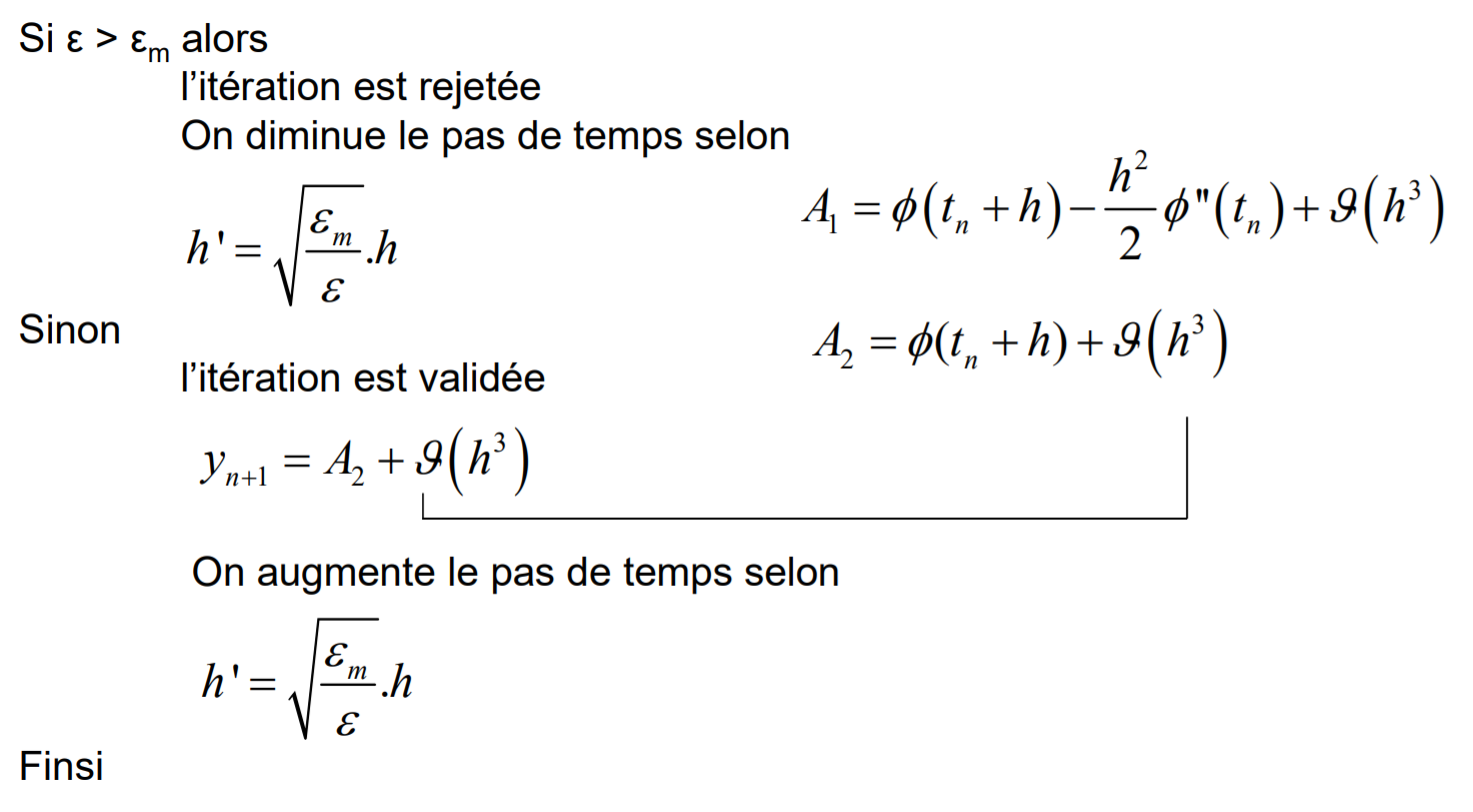
\includegraphics[height=8cm]{Algo_principe_Euler2pas.png} \\
  \caption{Algorithme de la méthode d'Euler à 2 pas}
    \label{ode12}
\end{figure}

\newpage
Une implémentation de l'algorithme en Matlab vous est présentée ci-dessous :

\matlabscript{rk_adapt12}{Implémentation de l'algorithme}

 \subsection{Méthode de Kutta -Merson}
 
   \begin{figure}[h!]
\centering
 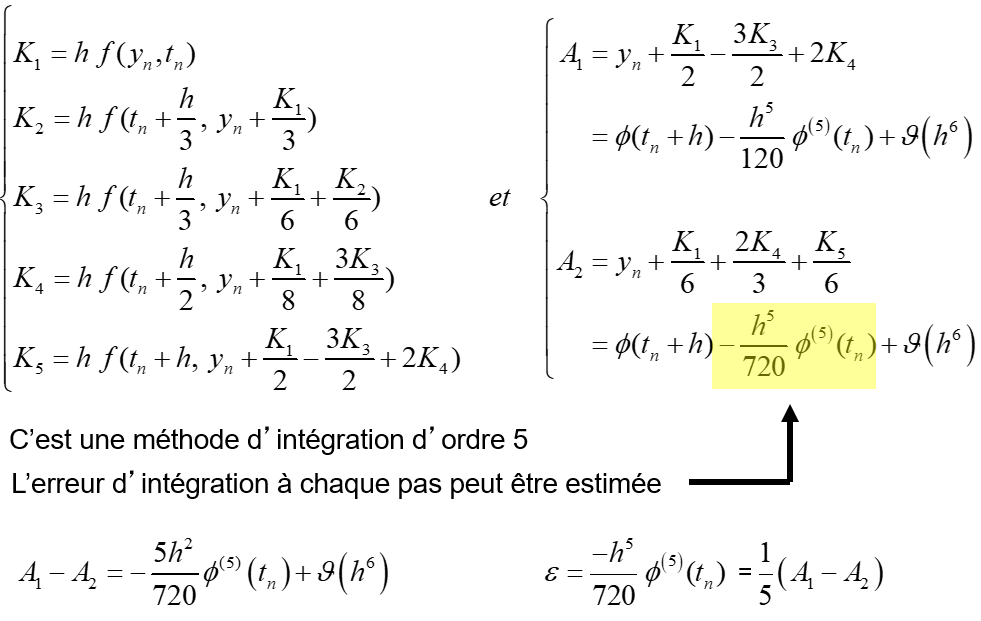
\includegraphics[height=8cm]{Kutta-Merson_fig1.png} \\
  \caption{Principe de la méthode de Kutta -Merson}
    \label{ode12}
\end{figure}

   \begin{figure}[h!]
\centering
 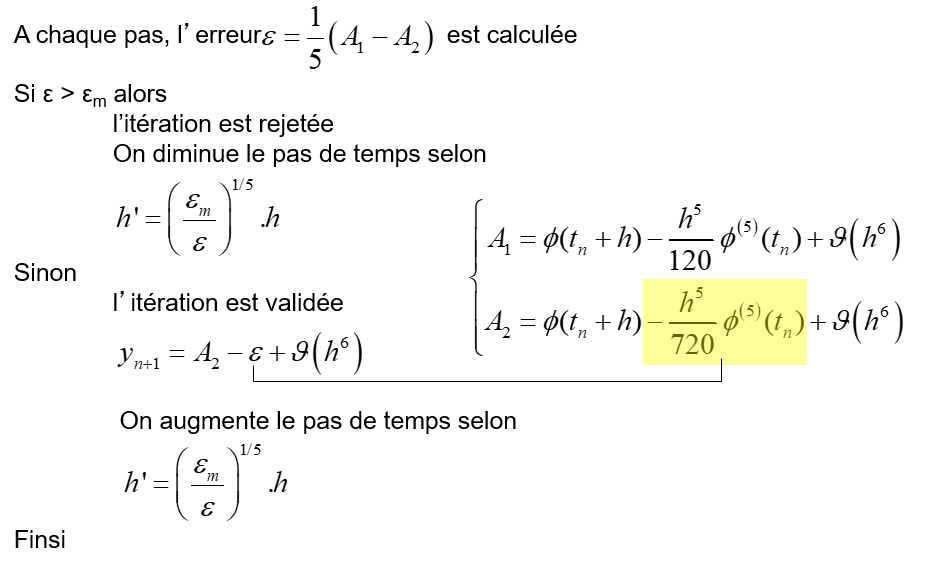
\includegraphics[height=8cm]{Kutta-Merson_fig2.png} \\
  \caption{Algorithme de la méthode de Kutta -Merson}
    \label{ode12}
\end{figure}

\newpage
\matlabscript{rkm}{Implémentation de la méthode de Kutta -Merson}
\end{document}

